\documentclass[a0paper, landscape, margin=0mm, innermargin=10mm,
     blockverticalspace=0mm, colspace=5mm, subcolspace=8mm]{tikzposter}
\tikzposterlatexaffectionproofoff

% define use package
\usepackage{graphicx}
\usepackage{xcolor}
\usepackage[utf8]{inputenc}
\usepackage[english]{babel}
\usepackage{natbib}

% new command
% this command will make blocks with custom height
\newlength\htblockbox
\newcommand{\mtblock}[3]{%
\block{#2}{%
\setlength{\htblockbox}{#1}%
\parbox[t][\htblockbox][c]{\linewidth}{#3}}}

% define image path
\graphicspath{ {./images/} }

% define custom color
\definecolor{mainColor}{RGB}{50,24,89}
\definecolor{sideColor}{RGB}{224,224,224}

% define color style
\definecolorstyle{uwoPosterStyle} {
 	\definecolor{colorOne}{named}{mainColor}
	 \definecolor{colorTwo}{named}{sideColor}
	  \definecolor{colorThree}{named}{white}
}{
% Background Colors
     \colorlet{backgroundcolor}{colorTwo}
     \colorlet{framecolor}{colorTwo}
     % Title Colors
     \colorlet{titlefgcolor}{colorThree}
     \colorlet{titlebgcolor}{colorOne}
     % Block Colors
     \colorlet{blocktitlebgcolor}{colorOne}
     \colorlet{blocktitlefgcolor}{white}
     \colorlet{blockbodybgcolor}{white}
     \colorlet{blockbodyfgcolor}{black}
     % Innerblock Colors
     \colorlet{innerblocktitlebgcolor}{white}
     \colorlet{innerblocktitlefgcolor}{black}
     \colorlet{innerblockbodybgcolor}{colorThree!30!white}
     \colorlet{innerblockbodyfgcolor}{black}
}

\definecolorstyle{uwoRefStyle} {
 	\definecolor{colorOne}{named}{mainColor}
	 \definecolor{colorTwo}{named}{sideColor}
	  \definecolor{colorThree}{named}{white}
}{
% Background Colors
     \colorlet{backgroundcolor}{colorTwo}
     \colorlet{framecolor}{colorTwo}
     % Title Colors
     \colorlet{titlefgcolor}{colorThree}
     \colorlet{titlebgcolor}{colorOne}
     % Block Colors
     \colorlet{blocktitlebgcolor}{colorOne}
     \colorlet{blocktitlefgcolor}{white}
     \colorlet{blockbodybgcolor}{white}
     \colorlet{blockbodyfgcolor}{white}
     % Innerblock Colors
     \colorlet{innerblocktitlebgcolor}{white}
     \colorlet{innerblocktitlefgcolor}{black}
     \colorlet{innerblockbodybgcolor}{colorThree!30!white}
     \colorlet{innerblockbodyfgcolor}{black}
}
\usecolorstyle{uwoPosterStyle}

% define title properties
\title{The Effect of Fearful Emotion on Selective Visuo-spatial Attention}
\titlegraphic{
\includegraphics{logo}}
\author{Student Name}
\institute{Department of Psychology, Faculty of Social Science, Western University, London, Ontario, Canada}

% define title arrangement
\makeatletter
\renewcommand\TP@maketitle{
    \begin{minipage}{0.2\linewidth}
       \centering
       \@titlegraphic
    \end{minipage}
   \begin{minipage}{0.7\linewidth}
        \centering
        \color{titlefgcolor}
        {\bfseries \Huge  \@title \par}
        \vspace*{1em}
        {\huge \@author \par}
        \vspace*{1em}
        {\LARGE \@institute}
    \end{minipage}
    \begin{minipage}{0.1\linewidth}
    	\centering
    	
\includegraphics[scale=0.7]{uwo}
    \end{minipage}
}
\makeatother

% define title style
\definetitlestyle{uwoTitleStyle}{
	width=1189mm, roundedcorners=0mm, linewidth=0mm, innersep=15mm,
	titletotopverticalspace=0mm, titletoblockverticalspace=10mm
}{
	\begin{scope}[line width=\titlelinewidth, rounded corners=\titleroundedcorners]
                         \draw[color=titlebgcolor, fill=titlebgcolor]
                             (\titleposleft,\titleposbottom) rectangle (\titleposright,\titlepostop);
                     \end{scope}
}

\usetitlestyle{uwoTitleStyle}

% define block style
\defineblockstyle{standardBlockStyle}{
     titlewidthscale=1, bodywidthscale=1,titlecenter,
     titleoffsetx=0pt, titleoffsety=0pt, bodyoffsetx=0mm, bodyoffsety=0mm,
     bodyverticalshift=0mm, roundedcorners=0, linewidth=2pt,
     titleinnersep=6mm, bodyinnersep=1cm
 }{
     \draw[color=framecolor, fill=blockbodybgcolor,
         rounded corners=\blockroundedcorners] (blockbody.south west)
         rectangle (blockbody.north east);
     \ifBlockHasTitle
         \draw[color=framecolor, fill=blocktitlebgcolor,
             rounded corners=\blockroundedcorners] (blocktitle.south west)
             rectangle (blocktitle.north east);
\fi }


\defineblockstyle{refBlockStyle}{
     titlewidthscale=1, bodywidthscale=1,titlecenter,
     titleoffsetx=0pt, titleoffsety=0pt, bodyoffsetx=0mm, bodyoffsety=5mm,
     bodyverticalshift=5mm, roundedcorners=0, linewidth=2pt,
     titleinnersep=6mm, bodyinnersep=1cm
 }{
     \draw[color=titlebgcolor, fill=titlebgcolor,
         rounded corners=\blockroundedcorners] (blockbody.south west)
         rectangle (blockbody.north east);
     \ifBlockHasTitle
         \draw[color=titlebgcolor, fill=titlebgcolor,
             rounded corners=\blockroundedcorners] (blocktitle.south west)
             rectangle (blocktitle.north east);
\fi }

% the begining of  the actual poster 
\begin{document}
	\maketitle
	\begin{columns}
		% first column
		\column{0.33}
		\useblockstyle{standardBlockStyle}
			
		% first blocks in column 1
		\block{ \textbf{\uppercase{Introduction}}}{
\setlength{\parindent}{8ex}
The modulation of selective visuospatial attention by fearful emotion is evolutionarily adaptive. In the present study, a modified version of the spatial cueing task was used to investigate the effect of fearful emotion on selective spatial attention. After invalid or valid location cued by a neutral or angry face, participants need to indicate the location of a target square. The results showed that the validity effect is mediated by emotion of the face. More specifically, response time is faster for the invalid condition compared with the valid condition in the fearful condition. These data suggested that fear emotion enhanced selective attention by ignoring irrelevant cueing information, which provides evidence for the effect of emotion on top-down spatial attention network. 		
		}
		
		% second block in column 1
		\block{\textbf{\uppercase{Keywords}}}{
Selective spatial attention, Top-down attention, Emotion, Fear, Spatial cueing task
		}
		
		% third block in column 1
		\mtblock{44.65cm}{\textbf{\uppercase{Method}}}{
			\textbf{Participants} \par
			\setlength{\parindent}{8ex}
			A total of 19 student from a cognitive research class in Western University were recruited as participants. The data from 18 students were included in the analyses. Data from one participant was excluded from final analyses due to irregularity (almost no corrected responses for invalid trials). Descriptive data of gender and age was not specified. \par
			\vspace{10mm}
			\noindent
			\textbf{Materials} \par	
			\setlength{\parindent}{8ex}
			\textbf{Modified Spatial Cueing Task. }The spatial cueing task is a modified vision to the study done by Vogt et.al (2008). The experiment was performed on LCD monitor and the experimental procedure was programmed by E-Prime software. All stimuli were presented against a black background. Two white rectangles (5.29 cm high × 2.59 cm wide) were placed on both side of the white fixation cross (5 mm high). A black square (1 cm) was served as a target for this task and placed 9.2 cm away from the fixation point in the white rectangles. Face pictures (fear or neutral) were presented as the same size of the rectangles. If the stimulus was presented at the same side with the target, it would be served as a valid cue. If the stimulus was presented at the opposite side, it would be served as an invalid cue. Reaction times were recorded in milliseconds. \par

			\textbf{Facial Picture Stimuli. }Face picture from Chinese Facial Affective Picture System (Gong, Huang, Wang, \& Luo, 2011) was used in this study for inducing emotion. A total of 148 angry faces and neutral faces were used to induce fearful and neutral emotion respectively. Both conditions have equal amounts of pictures for both genders. Neutral \& Angry face pictures have acceptance rates over 70\%. \par
			\vspace{12mm}
			\centering
			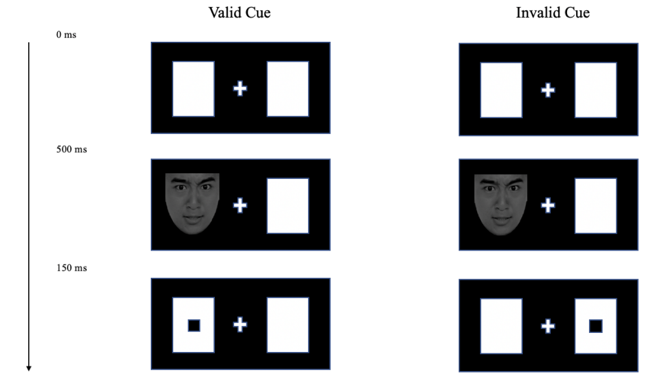
\includegraphics[scale=1.5]{procedure} \par
			\vspace{10mm}
			\noindent
			\raggedright
			\emph{Figure 1. }The example flowchart of the experiment procedure for valid and invalid condition with angry male face. \par
		}

		% second column
		\column{0.34}
			\mtblock{66.5cm}{\textbf{\uppercase{results}}}{
			\raggedright
			\textbf{Table 1}\par
			\emph {Mean reaction times (in ms) and corrected answer counts with their standard deviations (SD) for each combination of emotion (fear or neutral) and validity (invalid or valid) condition.} \par
			\centering
			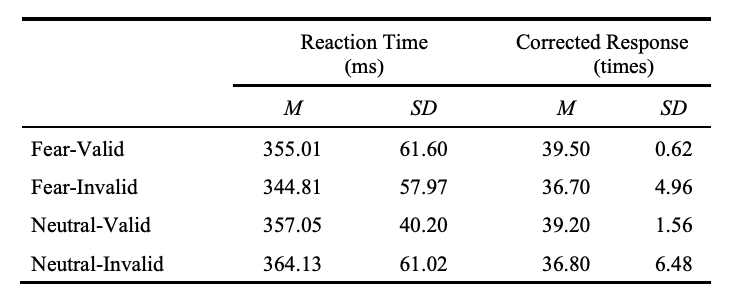
\includegraphics[scale=1]{table1}\par
			\raggedright
			\textbf{Table 2}\par
			\emph {Paired t-test results between different conditions with 95\% confidence intervals.}\par
			\centering
			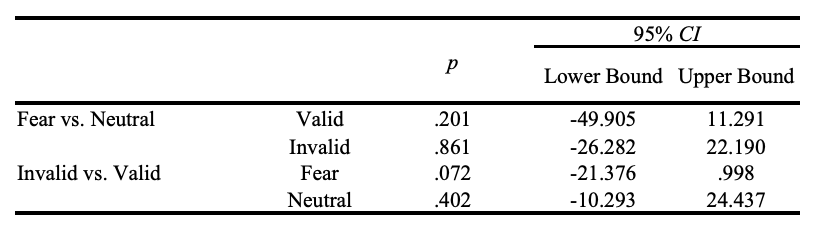
\includegraphics[scale=1]{table2}\par
			\vspace{2cm}			
			\centering
			\includegraphics[scale=1.8]{picture1}\par
			\raggedright
			\emph{Figure 2. }Mean response times (in ms) for each combination of emotion and validity conditions. (A) Bar graph of the mean reaction times for each condition with standard deviation. (B) An interaction effect of emotion and validity on reaction time with standard deviation. \par
			\vspace{2cm}
			\centering
			\includegraphics[scale=1.8]{picture2}\par
			\raggedright
			\emph{Figure 3.}. Mean corrected response counts on each combination of emotion and validity conditions with standard deviation. \par
			
			}
		% third column
		\column{0.33}
		
		% first block in column 3
		\block{\textbf{\uppercase{Discussion}}}{
		\setlength{\parindent}{8ex}
		\begin{itemize}
		\item The present study provided evidence that fearful emotion enhancing selective visuospatial attention. 
		\item Reaction time difference between invalid and valid condition was larger in fearful condition than neutral condition, which is consist with Easterbrook’s cue utilization theory (1959).  
		\item However, inconsistent with previous literature (Finucane, 2011), main effect of emotion was not found in the present study. 
		\item Although there was a trend that mean reaction time for fearful condition is faster than neutral condition, it did not reach statistical significance. 
		\item There is also no main effect of validity on reaction time. However, participants did have more corrected response in valid condition than invalid condition. 
		\end{itemize}
		}
		
		% second block in column 3
		\block{\textbf{\uppercase{Conclusion}}}{
		\setlength{\parindent}{8ex}
		In summary, fearful emotion affects selective visuospatial attention, more specifically, improves the subsequent searching of target due to ignoring of irrelevant information. The above results provide empirical evidence for the effect of the top-down processing of emotion on attention network and theoretical approaches on negative emotions. 
		}
		
		% reference block
		\usecolorstyle{uwoRefStyle}
		\useblockstyle{refBlockStyle}
		\mtblock{37cm}{\textbf{\uppercase{references}}}{
		% bibtex is an option, here is just for demonstration purpose
		\begin{enumerate}
		\item Armony, J. L., \& Dolan, R. J. (2002). Modulation of spatial attention by fear-conditioned stimuli: An event-related fMRI study. Neuropsychologia, 40(7), 817–826. \par
		\item Brosch, T., Sander, D., Pourtois, G., \& Scherer, K. R. (2008). Beyond Fear. Psychological Science, 	19(4), 362–370. \par
		\item Cohen, N., Henik, A., \& Mor, N. (2011). Can emotion modulate attention? Evidence for reciprocal links in the attentional network test. Experimental Psychology, 58(3), 171–179. \par 
		\item Davis, M., \& Whalen, P. J. (2001). The amygdala: Vigilance and emotion. Molecular
		Psychiatry, 6(1), 13–34. \par
		\item Easterbrook, J. A. (1959). The effect of emotion on cue utilization and the organization of behavior. Psychological Review, 66(3), 183–201. \par
		\item Finucane, A. M. (2011). The Effect of Fear and Anger on Selective Attention. Emotion, 11(4), 970–974. \par
		\item Fredrickson, B. L. (1998). What Good Are Positive Emotions? Review of General Psychology, 2(3), 300–319. \par
		\item Gable, P., \& Harmon-Jones, E. (2010). The motivational dimensional model of affect: Implications for breadth of attention, memory, and cognitive categorisation. Cognition and Emotion, 24(2), 322–337. \par
		\item Gong, X., Huang, Y.-X., Wang, Y., \& Luo, Y.-J. (2011). Revision of the Chinese Facial Affective Picture System. [Revision of the Chinese Facial Affective Picture System.]. Chinese Mental Health Journal, 25(1), 40–46. \par
		\item Katsuki, F., \& Constantinidis, C. (2014). Bottom-up and top-down attention: Different processes and overlapping neural systems. Neuroscientist, 20(5), 509–521. \par
		\item Miyazawa, S., \& Iwasaki, S. (2009a). Effect of negative emotion on visual attention: Automatic capture by fear-related stimuli. Japanese Psychological Research, Vol. 51, pp. 13–23. \par
		\end{enumerate}
		}
	\end{columns}
\end{document}
